\chapter{Software}
Nachfolgend wird das Design dieses Softwareprojekts dargestellt, sowie die leichte Erweiterung durch nachträgliche Module. Anschließend wird noch auf die bereits umgesetzten Module eingegangen und ihre Funktionsweise erklärt. 






\section{Design des Projektes mit CMake}


\subsection*{Ordnerstruktur}

Als Build System wird das plattformunabhängige Programmierwerkzeug CMake verwendet. Dieses Cross-Plattform Tool bietet einige Vorteile \cite{cmake.2018}:

\begin{itemize}
\item Erzeugung von Makefiles
\item Unterstützung verschiedener Compiler und Linker auf unterschiedlichen Plattformen
\item Unterstützung von System-Introspection
\item Erweiterbarkeit durch Makros
\end{itemize} 

Im folgenden wird die Ordnerstruktur dieses Projektes vorgestellt.

\textbf{include} Ordner: Dieser Ordner ist für die Header-Files zuständig. Unterteilt wird dieser Ordner zudem in die einzelnen umgesetzten Module (\textit{communication, motioncontrol, pathfinder, slam})

\textbf{launch} Ordner: Beinhaltet das ROS \textit{Launch File} für die Ausführung des Hector-SLAM Algorithmus

\textbf{scripts} Ordner: Beinhaltet nützliche Skripte, wie das zurücksetzen der erstellten Karte

\textbf{src} Ordner: Dieser Ordner ist für die Source-Files zuständig. Unterteilt ist dieser Ordner wieder in die einzelnen umgesetzten Module (\textit{communication, motioncontrol, pathfinder, slam})

\vspace{0.5cm}
\begin{lstlisting}
/include
	/communication
	/motioncontrol
	/pathfinder
	/slam
/launch
	hokuyo_hector_slam.launch
/srcipts
	resetMap
/src
	/communication
	/motioncontrol
	/pathfinder
	/slam
CMakeLists.txt
alf_main.cpp

\end{lstlisting}
\vspace{-0.5cm}

Im Hauptverzeichnis (ROOT) befinden sich die Hauptdatei (\textit{alf\_main.cpp}) sowie das \textit{CMakeLists.txt} in welcher die aktuelle Projektstruktur definiert ist. Insbesondere bei der Erweiterung dieses Projektes wäre es erdenklich, für jedes umgesetzte Modul ein eigenes CMake File anzulegen und im Root-Verzeichnis\textit{CMakeLists.txt} dann rekursiv die einzelnen CMake Files der Unterordner (Module) einzubinden. 


\subsection*{Umgesetzte Module}

Die bisherigen umgesetzten Module sind: 

\begin{itemize}
\item \textit{motioncontrol}: Modul für die Bewegungssteurung des ALF
\item \textit{pathfinder}: Modul für die Wegfindung 
\item \textit{slam}: Modul für die Interaktion mit dem SLAM Algorithmus

\item \textit{communication, lidar\_connect}: Modul für eine Server/Client-Verbindung, Modul für die Verbindung zum Lidar (Vorbereitet für die Verwendung für weiterführende Gruppen, jedoch in diesem Projekt nicht aktiv eingesetzt.
\end{itemize}

In den nachfolgenden Kapiteln werden die einzelnen Module genauer vorgestellt. 












\section{Verbindung zum Lidar}

Der Lidar Sensor ist direkt via USB mit dem Raspberry Pi 3b+ verbunden. Die Daten werden vom Lidar in Polarkoordinaten Darstellung geliefert. Um eine Karte aufbauen zu können, wurde ein Modul erstellt, das die Daten in kartesische Koordinaten transformiert. Somit ist es möglich nach jeder Messung des Lidars eine neue Karte mit der "`aktuellen Sicht"' des Sensors zu erstellen. Die Daten werden in einem Integer-Array gespeichert und können von einem SLAM Algorithmus verarbeitet werden . 

Das Modul verwendet zur Verbindung mit dem Lidar die unter der GNU GPL v3 stehende \href{https://github.com/simondlevy/BreezyLidar}{API "URG04LX"} \cite{breezylidar.2018}. Mit ihr ist es möglich einen kompletten Scan des Lidars aufzuzeichnen. 
\vspace{0.4cm}

\begin{lstlisting}
int data[MEASUREMENT_POINTS]; 
int measuredPoints;
URG04LX laser;

laser = URG04LX('dev/tty/ACM0')

measuredPoints = laser.getScan(data);

\end{lstlisting}
\vspace{-0.6cm}

Die Datenpunkte werden in polarkoordinaten Darstellung geliefert und müssen zur Weiterverarbeitung in kartesische Koordinaten umgerechnet werden. 

\begin{figure}[h]
\begin{center}
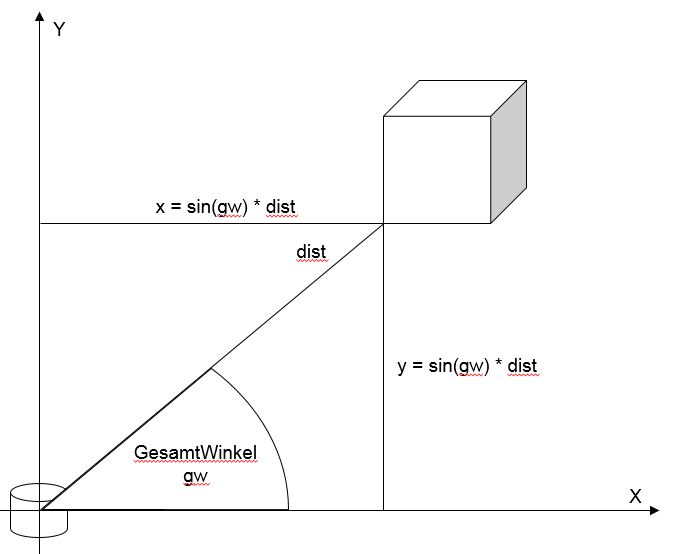
\includegraphics[width=10cm]{images/chapter5/LidarKoordRechnung.JPG}
\caption{Die Koordinaten berechnen}
\label{Koordinaten_errechnen}
\end{center}
\end{figure}

Die Umrechnung muss für alle aufgezeichneten Datenpunkte des Scans vorgenommen werden und liefert dann die Sicht des Lidars in einem Koordinatensystem:

\vspace{0.4cm}
\begin{figure}[h]
\begin{center}
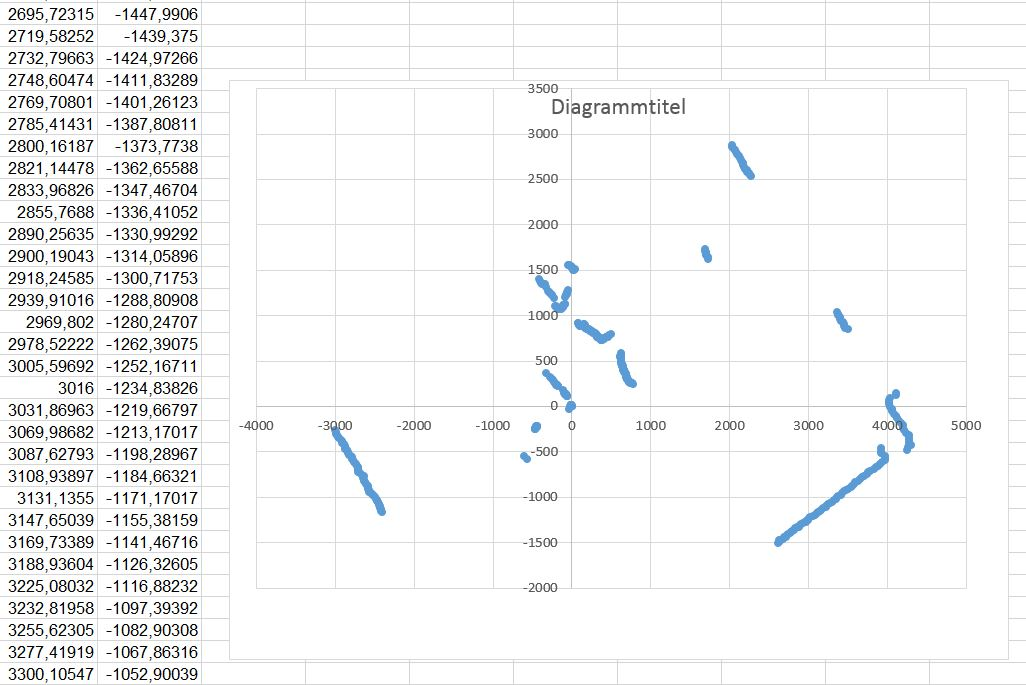
\includegraphics[width=10cm]{images/chapter5/kartKoord.JPG}
\caption{Koordinaten Veranschaulichung}
\label{Koordinaten_veranschaulichung}
\end{center}
\end{figure}



Das Modul wird momentan nicht verwendet, da der SLAM Algorithmus mit Hilfe von ROS realisiert wurde und die entsprechende Bibliothek einen eigenen Connector zum Lidar bereitstellt. Um folgenden Gruppen jedoch die Arbeit zu erleichtern, wurde das Modul trotzdem vorbereitet.











\section{Laser Scan Matcher als Odometrie Quelle}

Da zum aktuellen Zeitpunkt keine funktionierende Odometrie Quelle zur Verfügung steht, wird die Schätzung der Fahrzeugbewegung über einen Laser Scan Matcher realisiert. Ausführliche Dokumentation ist auf der ROS Wiki Seite verfügbar \href{http://wiki.ros.org/laser_scan_matcher}{Laser Scan Matcher}. Als Input dient wieder das \textit{/scan} Topic. Als Ausgabe erhält man die Position im \textit{/pose2D} Topic als x, y, $\theta$ Koordinaten. Diese Koordinaten werden dann anderen Modulen zur Verfügung gestellt. 









\section{SLAM}

Um eine SLAM Karte aufzubauen wurde erstmal eine Verbindung zum Hokuyo Lidar aufgebaut. Da bereits ein funktionierender ROS-Treiber vorhanden ist, konnte dieser übernommen werden. Dieser stellt ein neues Topic \textit{/scan} zur Verfügung, welches dann als Eingangspunkt für den SLAM verwendet wird. 

Um eine Map zu erhalten, wurde sich für den \href{http://wiki.ros.org/hector_mapping}{Hector-SLAM} entschieden. Dieser benötigt zum einen ein Topic auf dem die Laserscans zur Verfügung stehen (\textit{/scan}), zum anderen muss der Transformationsbaum zwischen dem Frame \textit{map}, \textit{scanmatcher\_frame}, \textit{base\_link} sowie \textit{laser} korrekt sein.  




\subsection{Transformationsbaum}

Nachfolgend der visualisierte zusammenhängende Transformationsbaum. Dieser ist zwingend notwendig, damit das Topic \textit{/map} erstellt wird. 


\begin{figure}[hbtp]
\centering
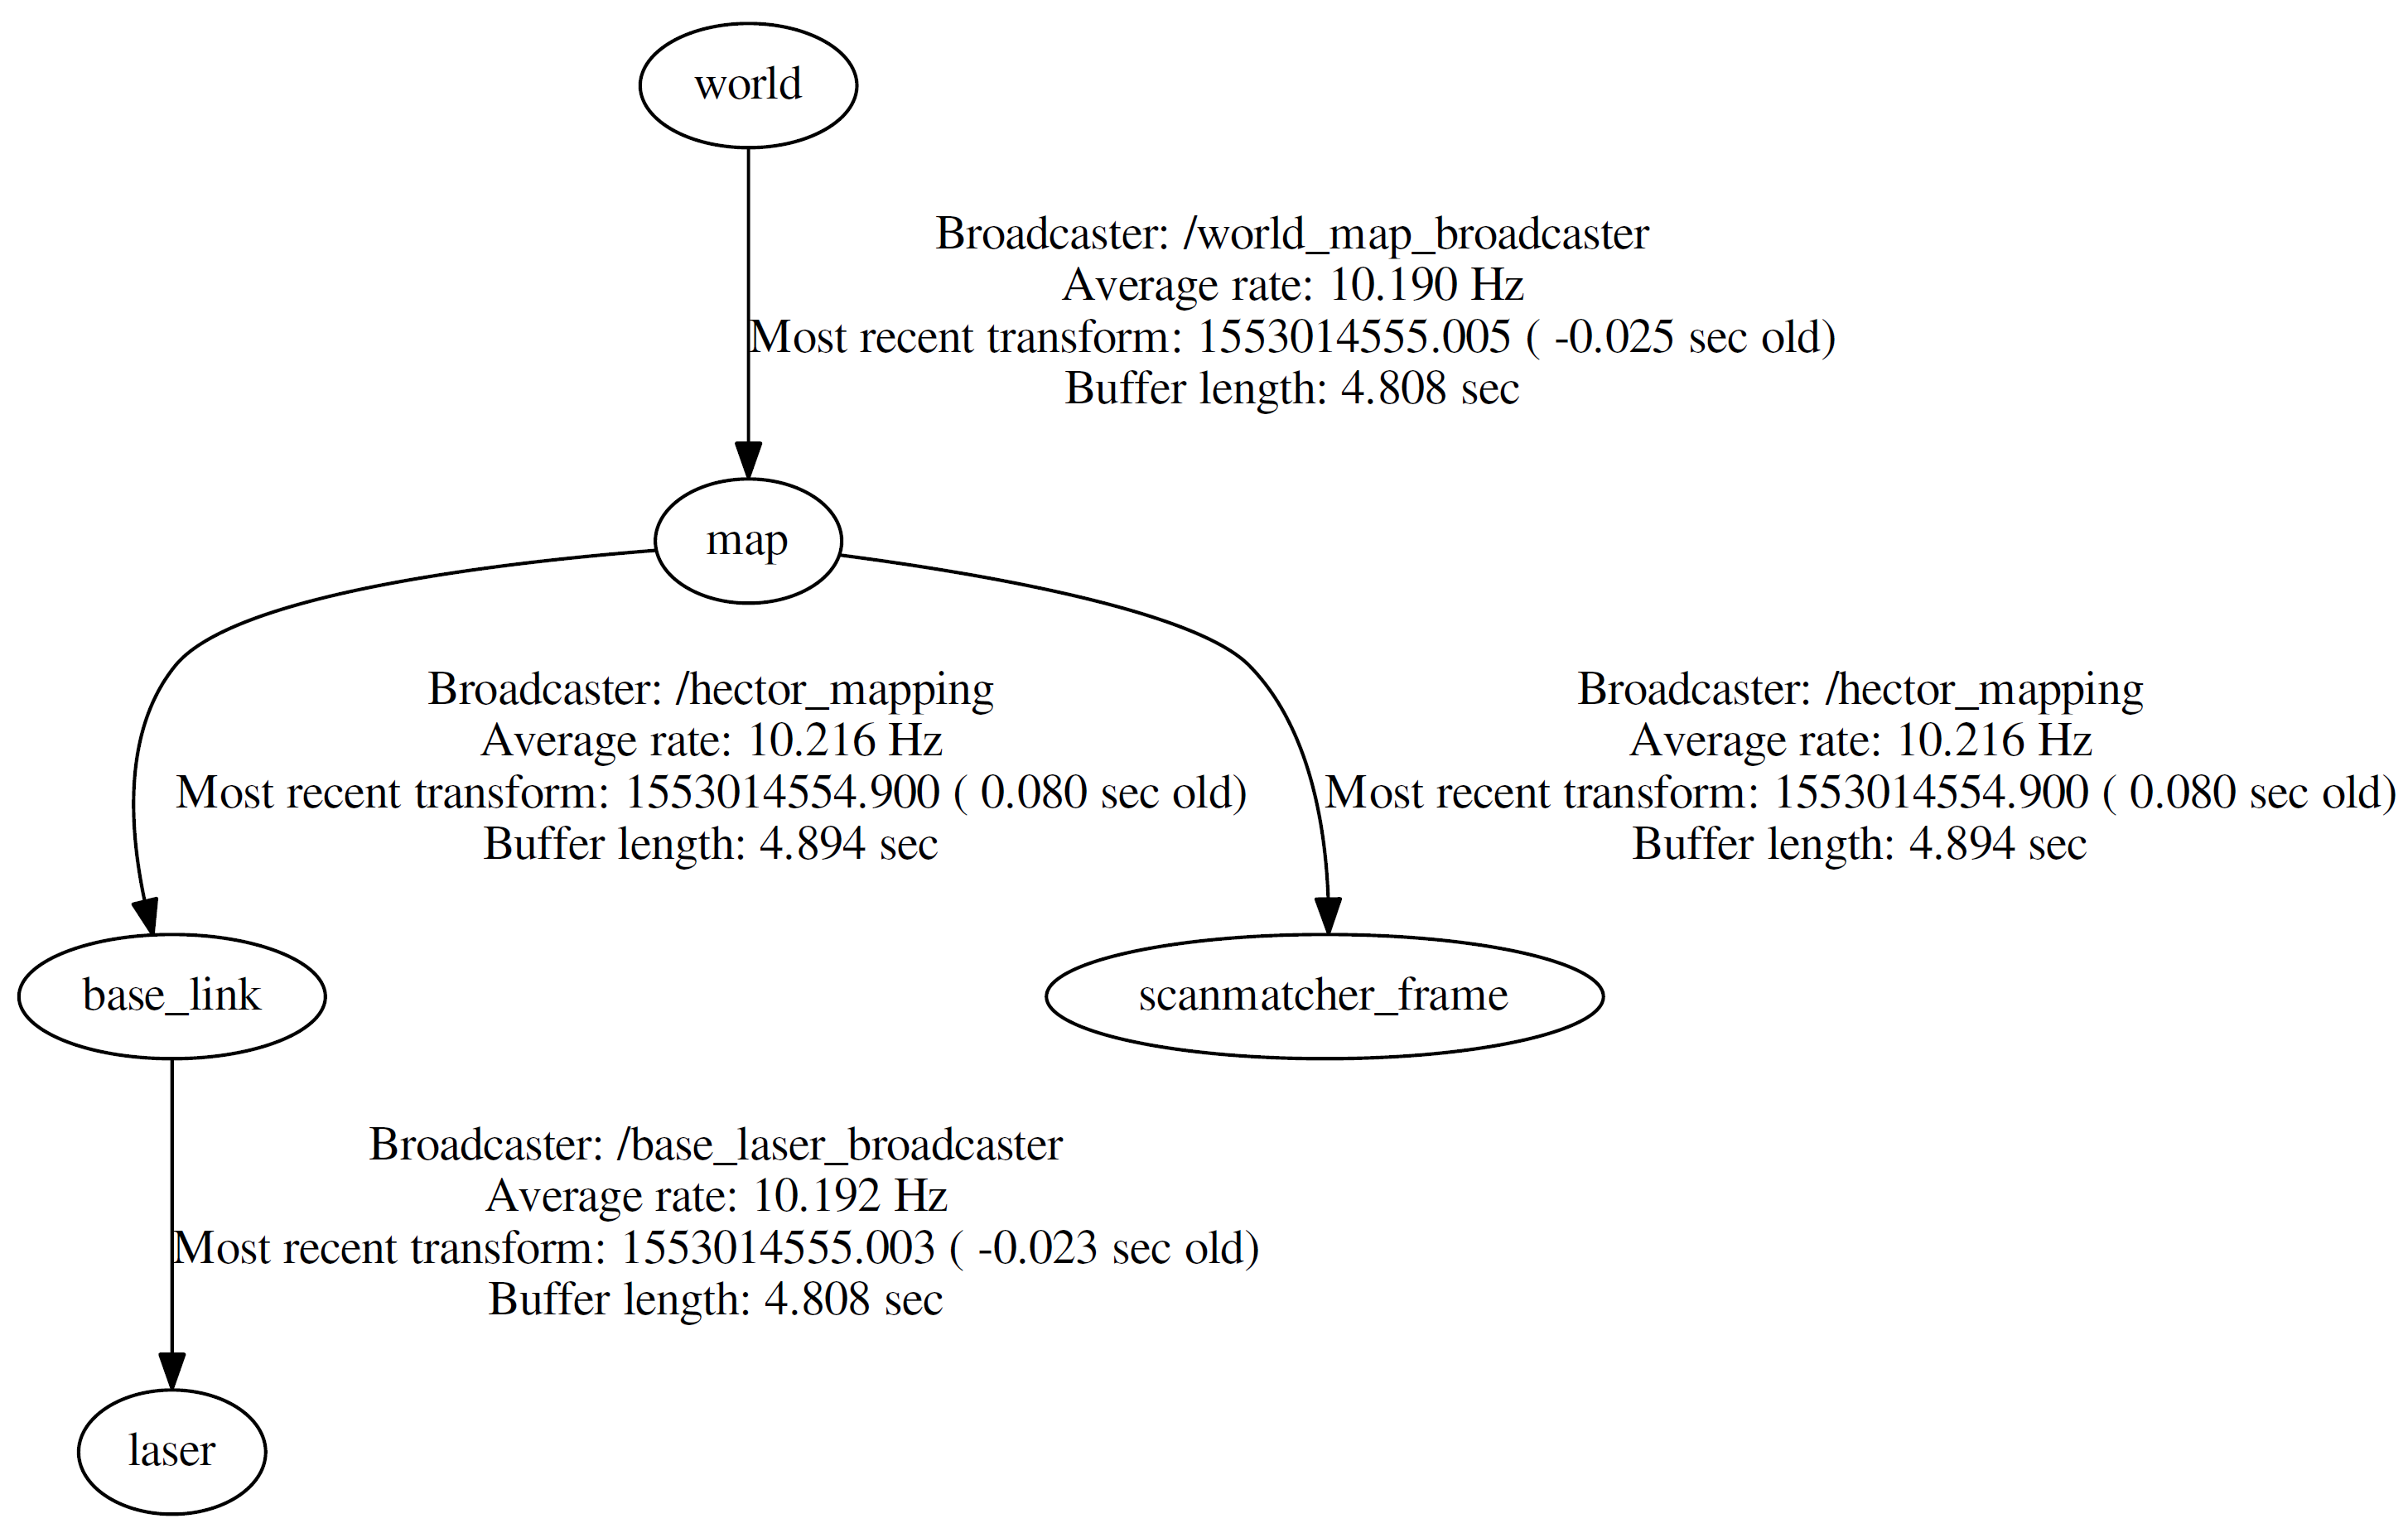
\includegraphics[scale=0.15]{images/chapter5/tf_alf.png}
\caption{Der aufgebaute Transformationsbaum}
\label{fig:tf_alf}
\end{figure}


Die Bedeutung der einzelnen Frames:

\begin{itemize}
\item \textbf{map}: Wird vom Hector-Slam erstellt und ist nötig für die Lokalisierung in der erstellten Map
\item \textbf{scanmatcher\_frame}: Wird vom Laser Scan Matcher erstellt und dient der relativen Positionsschätzung
\item \textbf{base\_link}: Wird auf den Schwerpunkt des ALF gelegt
\item \textbf{laser}: Wird vom Hokuyo Lidar Treiber erstellt
\end{itemize}



\subsection{Interface Modul für den SLAM}

Um auch ohne das Framework ROS die erstellte Karte zu erhalten, wurde ein Interface Modul erstellt. Mit diesem kann man auf definierte Membervariablen zugreifen und erhält so diverse Informationen vom SLAM-Algorithmus sowie der aufgebauten Karte. Die Karte wird dabei in einem Vektor mit Werten zwischen 0 und 255 abgespeichert und kann zur beliebiger Zeit abgefragt werden. 













\section{Wegefindung}

\textbf{Vorüberlegung:}

Das definierte Ziel ALF autonom einen Raum erkunden zu lassen, beinhaltet neben dem Erstellen einer Karte auch eine Wegberechnung zu unbekannten Flächen im Raum, die noch nicht vom Lidar erfasst wurden. Somit muss basierend auf der vom SLAM erstellten Karte ein Pfad zu den unbekannten Flächen gefunden werden.
Zu berücksichtigen ist, dass ALF durch seine Lenkung einen eingeschränkten Aktionsradius hat und es nicht möglich ist aus einer Geradeaus-Fahrt einen spitzen Winkel einzuregeln. Der maximale Lenkwinkel beträgt 45° und muss in die Routenplanung mit einbezogen werden. 

Eingabe: 
\begin{itemize}
\item Karte als Matrix
\item Egoposition auf Karte
\end{itemize}


\subsection{Datenschnittstelle zu SLAM Modul}

Die vom SLAM erhaltenen Daten entsprechen der einer PGM-Datei. In einem 2-dimensionalen Integer-Array wird die erstellte Karte als Grauwerte übergeben. 

Mögliche Werte sind:
\begin{itemize}
\item erkanntes Objekt (Schwarz)
\item Unbekannte Fläche (Grau)
\item Freifläche (Weiß)
\end{itemize}

\vspace{0.5cm}

Beispiel: 
\begin{lstlisting}
[ 127 127 127 127 127 127 127 ... ]
[ 127 127 127 127 127 127 127 ... ]
[ 127  0   0   0   0  127 127 ... ]
[ 127  0  255 255 255 127 127 ... ]
[ 127  0  255 255 255 127 127 ... ]
[ 127  0  255 255 255 127 127 ... ]
[ 127  0  255 255 255 127 127 ... ]

0 = erkanntes Objekt
127 = unbekannte Flaeche
255 = Freiflaeche
\end{lstlisting}


\subsection{Bereinigung der Karte}

Die vom SLAM erhaltene Karte kann unter Umständen nicht nur Schwarze, Weiße und fest definierte, graue Punkte enthalten. Je nach verwendetem SLAM werden für Messpunkte, die nicht sicher als Objekt oder Freifläche definiert werden können, als Zwischengrauwert angegeben. Dies führt jedoch bei der weiteren Berechnung des Pfades zu Problemen. Daher wurde eine Grenze definiert, die entscheidet, ob ein Grauwert als Freifläche oder Objekt betrachtet wird. Somit kann im weiteren Programm von bereinigten Werten (Objekt, Freifläche, Unbekannt) ausgegangen werden. 

\begin{figure}
    \subfigure[Karte mit ungenauen Messpunkten]{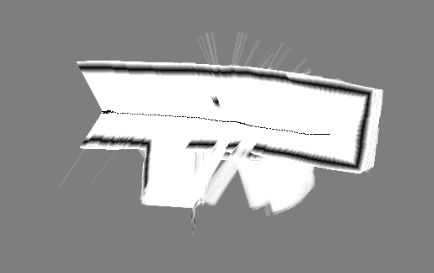
\includegraphics[width=0.49\textwidth]{images/chapter5/MapRegular.png}}
    \subfigure[Karte mit bereinigten Punkten]{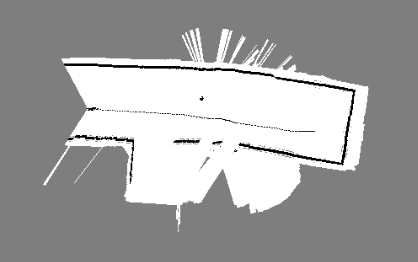
\includegraphics[width=0.49\textwidth]{images/chapter5/MapWhited.png}}
\caption{Vergleich vor und nach Bereinigung der Grauwerte}
\label{fig:ungenaueKarte}
\end{figure}


\subsection{Flächengewichtung}
\label{sec:gewichtung}

Zur Realisierung der in der Einleitung genannten Lenkwinkel-Problematik, wurde die Karte mit selbst definierten Grauwerten eingefärbt. Je weiter das Fahrzeug von einem Gegenstand bzw. einer Wand entfernt ist, desto unkritischer wird die Navigation bezüglich des Lenkwinkels.
Freiflächen in der Karte, die nahe an einer Wand liegen, sollen nach Möglichkeit gemieden werden. Punkte, die in der Mitte eines Raumes ohne Gegenstände liegen, werden als positiv für die Routenplanung angesehen. 
Somit sollte der Pfad immer zuerst in die Mitte eines Raumes führen und sich erst am Zielpunkt wieder einer Wand nähern. 
Umgesetzt wurde dies mit einer Grau-Gradientenfüllung der Karte, die später bei der Pfadberechnung als Gewichtung dienen. Die Freiflächenpunkte nahe einer Wand wurden mit einem hohen Gewicht (repräsentiert durch "dunkelgrau") belegt und verringern ihr Gewicht, je weiter sie von einer Wand entfernt liegen. 

\begin{figure}
    \subfigure[Karte mit bereinigten Punkten]{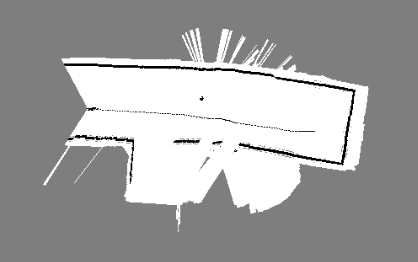
\includegraphics[width=0.49\textwidth]{images/chapter5/MapWhited.png}}
    \subfigure[Karte mit Gradientenfüllung]{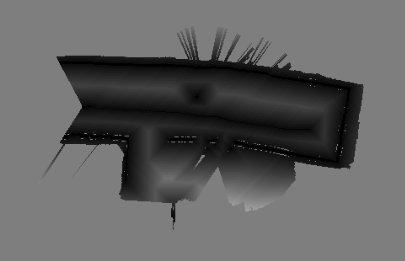
\includegraphics[width=0.49\textwidth]{images/chapter5/MapRemarked.png}}
\caption{Gradientenfüllung einer Karte basierend auf bereinigter Map}
\end{figure}



\subsection{Umwandlung in Graphen}

Um auf der bestehenden Karte einen Pfad berechnen zu können, muss die Matrix in einen Graphen überführt werden. Die einfachste (wenn auch nicht die performanteste) Methode war es jeden Freiflächen-Messpunkt des Lidars als eigenen Knoten anzusehen, der eine Verbindung zu den jeweilig benachbarten Messpunkten/Knoten hat. Als Kantengewicht wurde der entsprechende Grauwert des Nachbarknoten gewählt. Somit werden Pfade auf Freiflächen belohnt (Kantengewicht = 0) und Annäherungen an Gegenstände bestraft (Kantengewicht = steigender Grauwert). 
Für unbekannte Flächen sowie erkannte Objekte wurden keine Knoten in den Graphen eingefügt und diese auch nicht als Nachbarn angesehen. 

\vspace{0.5cm}
\begin{figure}[h]
\begin{center}
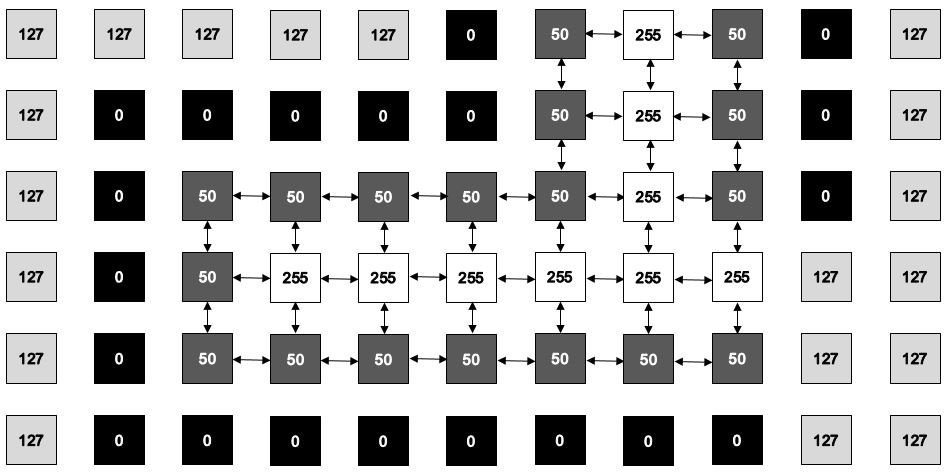
\includegraphics[width=15cm]{images/chapter5/GraphKnoten.JPG}
\caption{aus Map erstellter Graph}
\label{Map_aus_Graph}
\end{center}
\end{figure}


Dass aus jedem Pixel ein eigener Knoten wird, hat zur Folge, dass es extrem viele mögliche Pfade zu berechnen gibt. Hier existiert noch ein mögliches Verbesserungspotential für weitere Gruppenarbeiten. Da es sich jedoch um einen ersten autonomen Prototypen handelt, reicht die Umsetzung auf diesem Wege aus.




\subsection{Mögliche Ziele definieren und finden}
\label{sec:ziele}

Als Voraussetzung wird immer angenommen, dass die aktuelle Position des Fahrzeugs auf einer erkannten Freifläche liegt. Das übergeordnete Ziel einen Raum vollständig autonom zu erkunden, lässt sich nur erreichen, indem das Fahrzeug nicht zufällig durch den Raum fährt, sondern gezielt unbekannte Flächen ansteuert. Mögliche Ziele sind somit alle Übergänge von Freifläche zu unbekannter Fläche. 

Probleme:
Es kann passieren, dass der Lidar Sensor durch Reflektionen spiegelnder Oberflächen fehlerhafte Werte liefert. Somit entsteht bei der Verarbeitung der Daten mit dem SLAM der Eindruck, dass eine Freifläche hinter einer Wand erkannt wurde (siehe Abbildung \ref{fig:ungenaueKarte}). Da es auch dort zu Übergängen zwischen Freifläche und Unbekanntem Bereich kommen kann, werden diese Punkte auch als mögliche, zu erkundende Ziele erkannt. Da es jedoch keinen Weg zu diesen separierten Freiflächen gibt, ist es nicht möglich einen Pfad zu berechnen. Da sich dies als großes, nur sehr schwierig zu lösendes Problem herausstellte, wurde als Workaround die Pfadsuche so implementiert, dass alle Ziele durchgetestet werden und die Pfadberechnung nur abgeschlossen ist, wenn ein gültiger Pfad gefunden werden konnte.


\begin{figure}[h]
\begin{center}
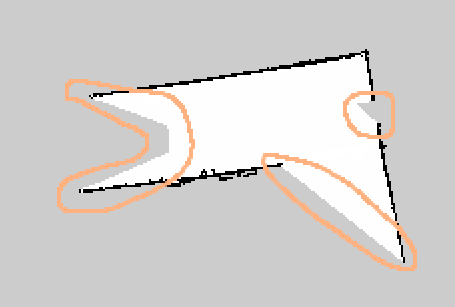
\includegraphics[width=15cm]{images/chapter5/MapUebergaenge_Markiert.png}
\caption{potentielle Ziele markiert}
\label{Map_aus_Graph}
\end{center}
\end{figure}



\subsection{Dijkstra}


Der erstellte Graph kann nun mit Hilfe eines Dijkstra-Algorithmus den kürzesten Weg von der Egoposition zum einem der 
\hyperref[sec:ziele]{\textcolor{blue}{möglichen, erkannten Ziele}} errechnen. Die \hyperref[sec:gewichtung]{\textcolor{blue}{zuvor eingeführte Gewichtung}} der Kanten führt nun dazu, dass ein Weg z.B. in der Mitte eines Ganges entlang errechnet wird. Bei 90° Winkeln wird eine leichte Biegung errechnet. Die Kantengewichtung ist auf dem kürzeren Pfad zwar schlechter, jedoch ist der Weg kürzer. Somit wird auch die Lenkwinkelproblematik entschärft. 

Als Dijkstra-Implementierung wurde die \href{https://gist.github.com/vertexclique/7410577}{Veröffentlichung von Mahmut Bulut} als Grundlage verwendet und für das Projekt angepasst \cite{dijkstra.2018}.



\subsection{Erstellter Pfad}

Als Ergebnis des Dijkstra-Algorithmus wird ein Pfad von der Egoposition über die Freiflächen bis hin zu einer zufälligen, unbekannten Fläche erzeugt. Die Navigation des Fahrzeuges übernimmt das Bewegungssteuerungsmodul. Sobald das Ziel erreicht wurde, kann ein neuer Pfad zu den noch verbleibenden, unbekannten Flächen erzeugt werden.


\subsection{Laufzeitoptimierung}

Der verwendete SLAM liefert eine Auflösung von 0.05m / Pixel. Zur Berechnung eines Pfades ist diese Auflösung jedoch zu detailiert, sodass die gesamte Karte in Blocks mit Freiflächen eingeteilt werden kann. Um die Laufzeit des Dijkstra zu verringern, wurde nicht jeder Pixel als Knoten angesehen, sondern ein Block von z.B. 5x5 Pixeln als 1 Knoten. Dies verringert zwar die Genauigkeit des Pfades, durch die Lenkwinkelproblematik wird diese jedoch sowieso nicht benötigt.

Ausgabe:
\begin{itemize}
\item Pfad von Egoposition zu Freifläche
\end{itemize}










\section{Bewegungssteuerung}

\subsection{Datenstruktur}

Die Bewegungssteuerung wandelt den berechneten Pfad der Wegefindung in Befehle für das Interface Board (\ref{sec:InterfaceBoard}) um. Der Pfad besteht aus Wegpunkten, die einzeln nacheinander angefahren werden. Die grundlegende Anfahrt eines Wegpunktes wird dabei über einzelne Befehle an das Interface Board übermittelt (Semantik: \texttt{[Lenkwinkel];[Fahrtrichtung];[Geschwindigkeit]}). Die Kommunikation erfolgt technisch über eine C - Datenstruktur, die sowohl im Bewegungssteuerungsmodul, als auch auf dem Interface Board identisch definiert ist. Die Datenstruktur kann per SPI vom Raspberry Pi aus regelmäßig auf das Interface Board übermittelt werden, um sowohl die Messdaten des Interface Boards zu lesen, als auch Befehle auf das Interface Board zu schreiben. Für dieses Projekt wurde eine Zykluszeit von 200ms gewählt, in der der Raspberry Pi 3b+ die Datenstruktur mit dem Interface Board synchronisiert. Tabelle \ref{tab:COMStructureType} zeigt den genauen Aufbau der Datenstruktur.

\begin{table}
\texttt{
\begin{tabular}{|c|c|p{6cm}|}
\hline 
\rule[-1ex]{0pt}{2.5ex} Datentyp & Name & Beschreibung \\ 
\hline 
\rule[-1ex]{0pt}{2.5ex} uint8 & CurrentSteeringMode & aktueller Betriebsmodus des Interface Boards \\ 
\hline 
\rule[-1ex]{0pt}{2.5ex} uint16 & CurrentSteeringSpeed & Fahrmotordrehzal (PWM von 0 bis 1000) \\ 
\hline 
\rule[-1ex]{0pt}{2.5ex} uint8 & CurrentSteeringDirection & Drehrichtung des Fahrmotors (0: rückwärts, 1: vorwärts) \\ 
\hline 
\rule[-1ex]{0pt}{2.5ex} float32 & CurrentSteeringAngle & Winkel des Lenkservos in Grad (-90.0 bis 90.0) \\ 
\hline 
\rule[-1ex]{0pt}{2.5ex} float32 & Target\_X & X Zielkoordinate für den automatischen Betriebsmodus \\ 
\hline 
\rule[-1ex]{0pt}{2.5ex} float32 & Target\_Y & Y Zielkoordinate für den automatischen Betriebsmodus \\ 
\hline 
\rule[-1ex]{0pt}{2.5ex} float32 & CurrentOrientation & aktuelle Ausrichtung des Interface Boards in Grad \\ 
\hline 
\rule[-1ex]{0pt}{2.5ex} float32 & CurrentPositionX & aktuelle X Position des Interface Boards in m \\ 
\hline 
\rule[-1ex]{0pt}{2.5ex} float32 & CurrentPositionX & aktuelle Y Position des Interface Boards in m \\ 
\hline 
\rule[-1ex]{0pt}{2.5ex} uint16 & USDistanceFrontLeft & aktueller Abstand des Ultraschall Sensors vorne links in cm \\ 
\hline 
\rule[-1ex]{0pt}{2.5ex} uint16 & USDistanceFrontRight & aktueller Abstand des Ultraschall Sensors vorne rechts in cm \\ 
\hline 
\rule[-1ex]{0pt}{2.5ex} uint16                                                                                                                                                                                                                         & USDistanceRear & aktueller Abstand des Ultraschall Sensors hinten in cm \\ 
\hline 
\end{tabular}
}
\caption{Datenstruktur COMStructureType, zur Kommunikation zwischen Raspberry Pi und Interface Board}
\label{tab:COMStructureType}
\end{table}




\subsection{Algorithmus}

Grundlage für den Algorithmus zur Anfahrt eines Wegpunktes ist ein einfacher Zustandsautomat. Dieser arbeitet die zur Verfügung gestellten Wegpunkte nacheinander ab. Die folgenden Eingabedaten werden dazu verarbeitet:


\begin{itemize}
\item aktuelle Position ($x_{pos}$, $y_{pos}$, und Winkel $ \theta_{pos} $)
\item der Pfad, eine Liste von Wegpunkten der Form $ \{(x_1, y_1), (x_2, y_2), ..., (x_n, y_n)\} $
\item der aktuelle absolute Winkel zum Zielwegpunkt $\theta_{ziel}$, berechnet von der Fahrzeugposition aus zu den Zielkoordinaten
\item der kleinsten Winkeldifferenz zum Zielwinkel, berechnet aus der aktuellen Ausrichtung des Fahrzeugs $\theta_{pos}$ und dem Zielwinkel $\theta_{ziel}$
\end{itemize}


Der Winkel $\theta_{ziel}$ von der aktuellen Position $(x_n, y_n)$ zum Ziel wird zunächst absolut nach Gleichung  \ref{equ:AbsoluterZielwinkel} bestimmt.

\begin{equation}
\theta_{ziel} = atan2(y_n - y_{pos}, x_n - x_{pos})
\label{equ:AbsoluterZielwinkel}
\end{equation}


Anschließend wird der kleinste Winkel $\theta_{rel}$ (relativer Zielwinkel) von der aktuellen Ausrichtung des Fahrzeugs $\theta_{ziel}$ berechnet (siehe Gleichung \ref{equ:relativerZielwinkel}).


\begin{equation}
\theta_{rel} = \left\{
\begin{array}{ll}
(-\theta_{ziel} + \theta_{pos}) , & ((360 - \theta_{ziel} + \theta_{pos}) > 180) \wedge ((-\theta_{ziel} + \theta_{pos}) \leq 180) \\
(-\theta_{ziel} + \theta_{pos}) , & ((360 - \theta_{ziel} + \theta_{pos}) > 180) \wedge ((-\theta_{ziel} + \theta_{pos}) > 180) \\
(360 - \theta_{ziel} + \theta_{pos}), & sonst.
\end{array}
\right.
\label{equ:relativerZielwinkel}
\end{equation}


Zu beachten ist, dass die Winkel $\theta_{pos}$ und $\theta_{ziel}$ jeweils nur Werte im Intervall \\ $[-180.0, 180.0]$ annehmen dürfen. Negative Winkel stehen hierbei für eine Ausrichtung im Uhrzeigersinn (mathematisch negativ), positive Winkel für eine Ausrichtung gegen den Uhrzeigersinn (mathematisch positiv).

Entsprechend der Berechnungen der notwendigen Zielwinkel und Koordinaten wird der Zustandsautomat in Bild \ref{fig:Zustandsautomat} durchlaufen. Die einzelnen Zustände sind in Tabelle \ref{tab:ZustaendeBewegungssteuerung} aufgeführt. In jedem dieser Zustände wird eine Datenübertragung vom Raspberry Pi 3b+ zum Interface Board initiiert, um konstant die aktuelle Geschwindigkeit, den Lenkwinkel und die Fahrtrichtung zu synchronisieren.

\begin{table}
\texttt{
\begin{tabular}{|c|p{7cm}|}
\hline 
\rule[-1ex]{0pt}{2.5ex} STATE\_INIT & Initialzustand nach Programmstart \\ 
\hline 
\rule[-1ex]{0pt}{2.5ex} STATE\_SCAN & Drehen um die eigene z-Achse, 360.0° Erfassung der Lidar Karte \\ 
\hline 
\rule[-1ex]{0pt}{2.5ex} STATE\_FETCH\_PATHS & Erfassung des geplanten Pfades aus Datei \\ 
\hline 
\rule[-1ex]{0pt}{2.5ex} STATE\_GET\_NEXT\_WAYPOINT & nächsten Wegpunkt ermitteln \\ 
\hline 
\rule[-1ex]{0pt}{2.5ex} STATE\_TRAVEL & Fahren zum nächsten Wegpunkt \\ 
\hline 
\rule[-1ex]{0pt}{2.5ex} STATE\_REVERSE\_BACKWARD & Rückwärts Fahren und gleichzeitig drehen, um nächsten Wegpunkt zu erreichen \\ 
\hline 
\rule[-1ex]{0pt}{2.5ex} STATE\_REVERSE\_FORWARD & Vorwärts Fahren und gleichzeitig drehen, um nächsten Wegpunkt zu erreichen \\ 
\hline 
\end{tabular}
}
\caption{Übersicht über die Zustände der Bewegungssteuerung}
\label{tab:ZustaendeBewegungssteuerung}
\end{table} 

\begin{figure}[hbtp]
\centering
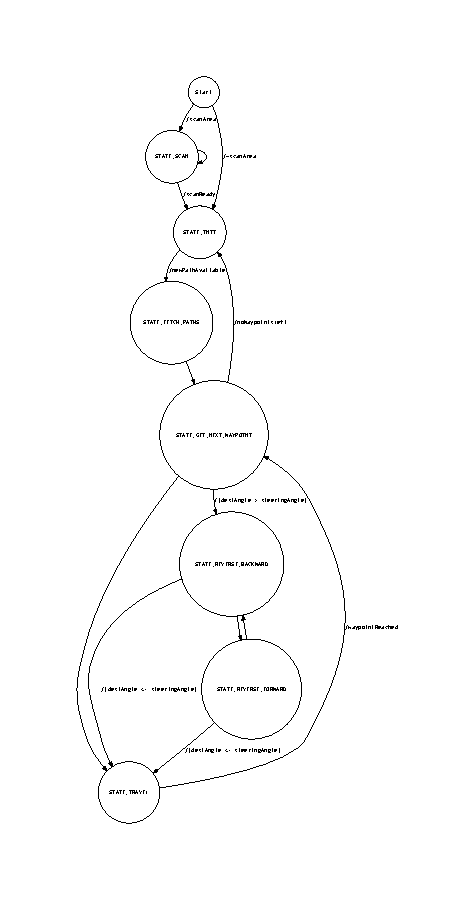
\includegraphics[scale=1.5]{images/chapter5/StateModel.pdf}
\caption{Zustandsautomat der Bewegungssteuerung}
\label{fig:Zustandsautomat}
\end{figure}